% !TeX root=main.tex

% Different Number of Ports
\begin{figure*}
	\centering
	\begin{minipage}[b]{.49\textwidth}
		% 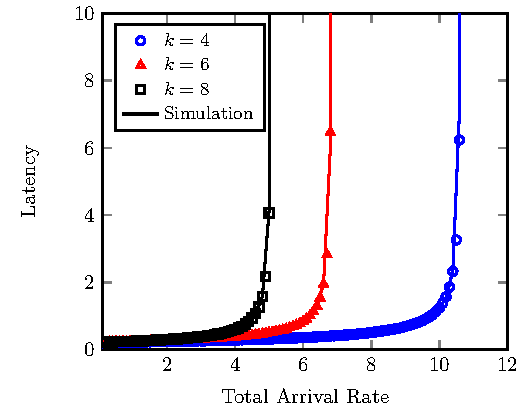
\includegraphics[width=\linewidth]{graphs/num_ports}
		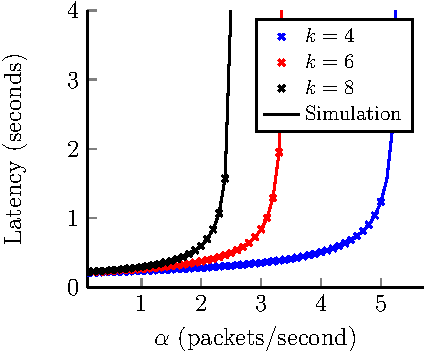
\includegraphics[width=\linewidth]{graphs/num_ports-crop}
		\caption{Latency predicted by the model and simulation for different numbers
		of ports ($N_s=1$, $K_i=2$, $k={8,16,24}$, $k_v=2$, $p_m=0$).}
		\label{fig:num_ports}
	\end{minipage}
	\hfill
	\begin{minipage}[b]{.49\textwidth}
		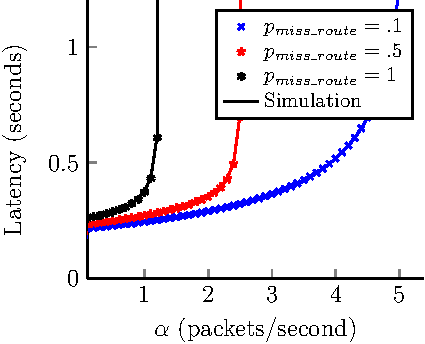
\includegraphics[width=\linewidth]{graphs/diff_sdn-crop}
		\caption{Latency predicted by the model and simulation for different miss rates ($N_s=1$, $K_i=2$, $k=4$, $k_v=2$, $p_m={0.1,0.5,1.0}$).}
		\label{fig:sdn_perc}
	\end{minipage}

	\vspace{2mm}

	\begin{minipage}[b]{.49\textwidth}
		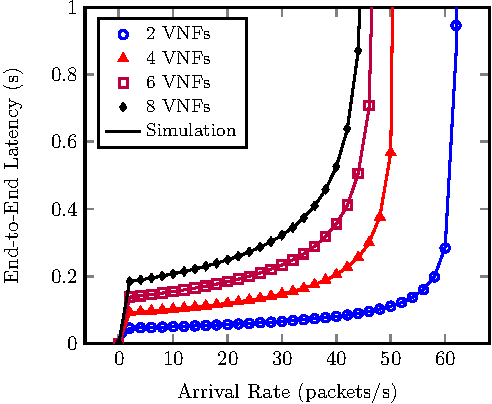
\includegraphics[width=\linewidth]{graphs/diff_lengths-crop}
		\caption{Latency predicted by the model and simulation for a single service with different lengths ($N_s=1$, $K_i={3,5,7,9}$, $k=4$, $k_v =2$, $p_m=0$).}
		\label{fig:length_chain}
	\end{minipage}
	\hfill
	\begin{minipage}[b]{.49\textwidth}
		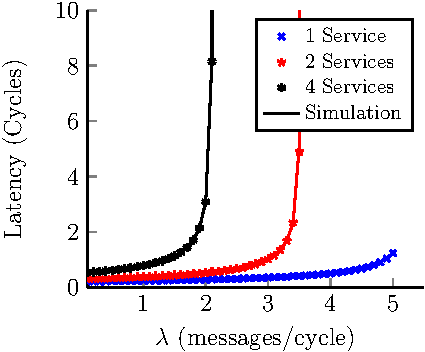
\includegraphics[width=\linewidth]{graphs/mult_services-crop}
		\caption{Latency predicted by the model and simulation for several services
		with different length service chains ($N_s={1,3,5}$, $K_i=3$, $k=4$, $k_v=2$, $p_m=0$).}
		\label{fig:mult_services}
	\end{minipage}

\end{figure*}

\section{Validation and Performance Analysis}
\label{sec:validation}

\subsection{Model Validation}

To verify the accuracy of the analytical model, a discrete event simulator has been built using OMNeT++ \cite{VargaH08} to simulate a NFV and SDN enabled datacentre network. Each simulation experiment was run until the network reaches its steady state where further network cycles do not change the collected statistics appreciably. In practice a datacentre can contain on the order of tens of thousands of servers \cite{AWS16}, with each switch supporting 1 to 100Gbits/s traffic a second. At high service rates, queue behaviour changes over very small intervals making it difficult to measure or demonstrate the accuracy of the results. Therefore, results from a scaled down version of a typical datacentre are presented in this work. Except where otherwise stated, the following parameters are used:

\begin{itemize}
	\item The number of ports $k = 8$, $k_{v} = 3$ and $p_{m} = 0$
	\item Each network component (switch/server, VNF and controller) can service 82 packets per second per port, \footnote{A 1Gb/s ethernet switch can process $\sim\!82000$ ethernet packets a second per port} ($\mu_{s}$, $\mu_{v}$ and $\mu_{c}$)
	\item Services are selected with equal probability
	\item The network provides 1 service with 5 VNFs ($N_s = 1$, $K_i = 5$)
\end{itemize}

Figs 2 to 5 depict the mean message latency predicted by the model plotted against those provided by the simulation experiments for a range of parameter settings. For the model, results are only shown where the network is in a steady state, i.e. where the arrival rate is lower than or equal to the service rate for all queues. The figures demonstrate that the simulation results closely match those predicted by the model. The tractability and accuracy of the analytical model make it suitable for analysis of next generation NFV and SDN enabled MCC datacentres.

\subsection{Performance Analysis}
We now show how the proposed analytical model can be a useful tool to optimise the design of an SDN and NFV enabled MCC datacenter network. We demonstrate the utility of the model for three key parameters: the scale of the network infrastructure, the table miss probability and the number and length of services.

\subsubsection{Impact of the size of the datacenter on the end-to-end latency}
The proposed analytical model can also be used to quantitatively analyse the relationship between latency and the size of the datacentre. From Fig. \ref{fig:num_ports} we can see that the Fat Tree scales as expected, with the increased number of VNFs in the network being balanced out by the increased service rate available at each switch. 

\subsubsection{Impact of the miss probability in SDN flow tables on the end-to-end latency}
The SDN paradigm provides the benefit of a simplified network management and centralised system optimisation. However, from the packet forwarding perspective, the centralised control incurrs extra transmission latency during packet delivery. The proposed analytical model allows us to investigate the relationship between the reliance on centralised control and the end-to-end latency of each service. Fig. \ref{fig:sdn_perc} shows that the system is only stable for low arrival rates when the SDN controller must frequently assist with routing instructions. Considering Eq. \ref{eq:arr_sdn}, we can see that the arrival rate at the SDN controller is proportional to the network traffic that is produced by the VNFs. Due to the total connectivity between the virtual machines and the SDN controller, even a slight increase of the traffic rate can overwhelm the SDN controller. To ensure that the SDN controller does not become a bottleneck in the system, network designers should ensure that routing tables at switches contain the majority of the information required for routing so that few requests must be sent to the controller, or ensure the processing capability of the SDN controller is sufficient to handle the traffic rate from the VNFs.

\subsubsection{Impact of the number and length of NFV services on the end-to-end latency}
Finally, we also consider the related situations of a different length services and of multiple services of varying lengths. As the datacenter network will be shared by multiple services to improve resource utilisation, it is important to investigate how these parameters impact the end-to-end latency. From Fig. \ref{fig:length_chain} we can observe the expected latency increasing as the length of the service increases. This is a consequence of the increased effective arrival rate that results from longer services (Eq. \ref{eq:effective_arrival}). In comparison, Fig. \ref{fig:mult_services} shows that increasing the number of services does not impact on the latency provided the expected arrival rate is distributed over the services. This indicates that the most important factor to consider when planning a datacentre is not the length or number of services, but the effective arrival rate of these two properties combined.